\documentclass[a4paper]{article}

\addtolength{\hoffset}{-2.25cm}
\addtolength{\textwidth}{4.5cm}
\addtolength{\voffset}{-3.25cm}
\addtolength{\textheight}{5cm}
\setlength{\parskip}{0pt}
\setlength{\parindent}{0in}

%----------------------------------------------------------------------------------------
%	PACKAGES AND OTHER DOCUMENT CONFIGURATIONS
%----------------------------------------------------------------------------------------

\usepackage{blindtext} % Package to generate dummy text
\usepackage{charter} % Use the Charter font
\usepackage[utf8]{inputenc} % Use UTF-8 encoding
\usepackage{microtype} % Slightly tweak font spacing for aesthetics
\usepackage[english]{babel} % Language hyphenation and typographical rules
\usepackage{amsthm, amsmath, amssymb} % Mathematical typesetting
\usepackage{float} % Improved interface for floating objects
\usepackage[final, colorlinks = true,
            linkcolor = black,
            citecolor = black]{hyperref} % For hyperlinks in the PDF
\usepackage{graphicx, multicol} % Enhanced support for graphics
\usepackage{xcolor} % Driver-independent color extensions
\usepackage{marvosym, wasysym} % More symbols
\usepackage{rotating} % Rotation tools
\usepackage{censor} % Facilities for controlling restricted text
\usepackage{listings} % Environment for non-formatted code, !uses style file!
\usepackage{pseudocode} % Environment for specifying algorithms in a natural way
 % Environment for f-structures, !uses style file!
\usepackage{booktabs} % Enhances quality of tables
\usepackage{tikz-qtree} % Easy tree drawing tool
 % Configuration for b-trees and b+-trees, !uses style file!
\usepackage[backend=biber,style=numeric,
            sorting=nyt]{biblatex} % Complete reimplementation of bibliographic facilities
\addbibresource{ecl.bib}
\usepackage{csquotes} % Context sensitive quotation facilities
\usepackage[yyyymmdd]{datetime} % Uses YEAR-MONTH-DAY format for dates
\renewcommand{\dateseparator}{-} % Sets dateseparator to '-'
\usepackage{fancyhdr} % Headers and footers
\pagestyle{fancy} % All pages have headers and footers
\fancyhead{}\renewcommand{\headrulewidth}{0pt} % Blank out the default header
\fancyfoot[L]{} % Custom footer text
\fancyfoot[C]{} % Custom footer text
\fancyfoot[R]{\thepage} % Custom footer text
\newcommand{\note}[1]{\marginpar{\scriptsize \textcolor{red}{#1}}} % Enables comments in red on margin
\usepackage{mathtools}
\usepackage{amsmath}
\DeclarePairedDelimiter\abs{\lvert}{\rvert}%
\usepackage{cancel}
\usepackage{minted}
\usepackage{float}
%-------------------------------

%----------------------------------------------------------------------------------------

%-------------------------------
%	ENVIRONMENT SECTION
%-------------------------------
\pagestyle{fancy}
\usepackage{mdframed}


\newenvironment{problem}[2][Problema]
    { \begin{mdframed}[backgroundcolor=gray!20] \textbf{#1 #2} \\}
    {  \end{mdframed}}

% Define solution environment
\newenvironment{solution}
    {\textit{Solución}}
    {}


%-------------------------------------------------------------------------------------------
%	CUSTOM COMMANDS
%-------------------------------
\newcommand{\gaussian}{\frac{1}{\sigma\sqrt{2\pi}}\exp\left(- \frac{(x-\mu)^2}{2\sigma^2}\right)}
\newcommand{\R}{\mathbb R}

\newtheorem{thm}{Teorema}
\newtheorem{lema}{Lema}

\newtheorem{ndef}{Definición}

\def\inline{\lstinline[basicstyle=\ttfamily,keywordstyle={}]}


\begin{document}


%-------------------------------
%	TITLE SECTION
%-------------------------------

\fancyhead[C]{}
\hrule \medskip % Upper rule
\begin{minipage}{0.295\textwidth}
\raggedright
\footnotesize
Francisco Javier Sáez Maldonado \hfill\\
77448344F \hfill\\
franciscojavier.saez@estudiante.uam.es
\end{minipage}
\begin{minipage}{0.4\textwidth}
\centering
\large
Take Home Exam 1\\
\normalsize
Optimización\\
\end{minipage}
\begin{minipage}{0.295\textwidth}
\raggedleft
\today\hfill\\
\end{minipage}
\medskip\hrule
\bigskip

%-------------------------------
%	CONTENTS
%-------------------------------
\section{Cuestiones}

\begin{problem}{1}
¿Cuáles son los criterios de parada del algoritmo simplex algebraico? Expón todas las alternativas posibles y las soluciones a que dan lugar.
\end{problem}

Para dar respuesta a este problema, recurrimos al document PDF en el que se detalla la versión algebraica del algoritmo simplex para problemas de minimización.\\

Como repaso muy breve de notación para entender la respuesta, recordamos que el problema debe estar expresado en forma estándar (restricciones de igualdad) y que se puede expresar como encontrar el mínimo de una función \(z = \mathbf{c}^T \mathbf{x}\) sujeto a unas restricciones que se escriben matricialmente como \(Ax = b\), siendo \(A\) una matriz y \(b\) un vector. Además, descompondremos \(A = (B \ N)\) siendo \(B\) la matriz básica y \(N\) la no básica.

Llamaremos \(I_N\) al conjunto de índices de las variables \textbf{no básicas}. Encontramos dos puntos en los que puede terminar este algoritmo.

\begin{enumerate}
\item Tras calcular para todas las variables no básicas los valores
\[
z_j - c_j = c_B B^{-1}a_j - c_j \quad \forall j \in I_N,
\]
y considerar \(z_k - c_k\) como el máximo de estos valores, el algoritmo \textbf{termina si} \(z_j - c_j \leq 0\), verificándose el \textbf{criterio de optimalidad simplex}, siendo la Solución Básica Factible (SBF) \textbf{óptima}. En esta parada, pueden darse dos posibles alternativas para las soluciones:
\begin{enumerate}
\item Si se verifica que \(z_j - c_j = 0\), entonces se tiene que tenemos \textbf{infinitas soluciones óptimas}.
\item Si, por el contrario, tenemos que \(z_j - c_j < 0\), entonces tenemos una solución \textbf{única} óptima.
\end{enumerate}

\item El algoritmo también para si, tras realizar el \emph{criterio de la razón mínima}, es decir, calcular
\[
\frac{\bar b_r}{y_{rk}} = \min_{1 \leq i \leq m} \left\{\frac{\bar{b_i}}{y_{rk}} \ : \ y_{ik} > 0\right\}  
\]
nos damos cuenta de que dicho valor mínimo \(\frac{\bar b_r}{y_{rk}} \) \textbf{no existe}. Entonces, el algoritmo termina y el problema tiene \textbf{solución no acotada}.
\end{enumerate}


\begin{problem}{2}
  Una forma alternativa de definición de problemas de programación lineal viene dada por el modelo dual. En esta cuestión se pide que definas cuál es el Problema Dual de un Problema Primal.
  \begin{enumerate}
\item ¿Qué relación existe entre ambos en términos de las soluciones posibles?
\item ¿Ofrece alguna ventaja la formulación dual respecto de la primal?
  \end{enumerate}
\end{problem}
\emph{}
Para cada problema de programación lineal, \(P\) (Primal), existe otro problema de programación lineal asociado a este, \(D\), llamado el problema dual. Según si nuestro problema primal \(P\) está en forma estándar o canónica, tenemos un problema dual asociado, aunque las formulaciones duales son equivalentes entre sí, independientemente de cómo esté formulado nuestro problema primal \(P\). Asumiremos que nuestro problema primal está escrito en forma canónica.\\

Si nuestro \textbf{problema primal} \(P\) es el siguiente:
\begin{align*}
\text{P : Minimize }  cx &\\
\text{subject to } Ax & \geq b\\
 x & \geq 0
\end{align*}
entonces, su \textbf{problema dual} \(D\) asociado es 
\begin{align*}
  \text{D : Maximize }  wb &\\
  \text{subject to }  wA & \leq c\\
   w & \geq 0
\end{align*}

Como el problema dual es también un problema de programación lineal, se tiene además el siguiente lema:

\begin{lema}
El problema dual \(D'\) del problema dual \(D\), es el problema primal \(P\) del problema dual \(D\). (\emph{Propiedad involutiva.})
\end{lema}

Vamos a comentar las \textbf{relaciones más importantes} en términos de las soluciones posibles. El primer resultado que debemos comentar es el siguiente

\begin{thm}[Teorema de dualidad débil.]
Para cualquier posible solución factible del problema primal \(P\), el valor de la función objetivo es siempre mayor o igual que el valor de la función objetivo en el problema dual \(D\). 
\end{thm}

Además, introducimos un lema que nos llevará al teorema final que relacionará las soluciones de ambos problemas:

\begin{lema}
Si uno de los problemas posee una solucion óptima, entonces \textbf{ambos problemas poseen} soluciones óptimas y los valores de la función objetivo óptimos son iguales.
\end{lema}

Gracias a este lema y a otra serie de resultados, llegamos al siguiente teorema:

\begin{thm}[Teorema de dualidad fuerte.]\label{th:dual}
En relación a las soluciones del problema primal \(P\) y su dual \(D\), se cumple \textbf{exactamente uno} de los siguientes:
\begin{enumerate}

\item Ambos poseen soluciones óptimas \(\mathbf{x}^*, \mathbf{w}^*\) con \(\mathbf{c}\mathbf{x}^* = \mathbf{w}^*\mathbf{b}\).
\item Un problema tiene solución óptima no acotada, por lo que el otro problema no tiene solución factible.
\item Ninguno tiene solución factible.
\end{enumerate}
\end{thm}


Podemos hablar por último de las \textbf{posibles ventajas} que ofrece usar la formulación dual respecto del problema original.

\begin{itemize}

\item Una primera clara ventaja que podría darnos se da cuando tenemos muchas variables \(x_i\) y pocas restricciones \(a_i\), pues en ese caso al obtener el problema dual conseguimos un problema sencillo (con menos variables objetivo \(w_i\)) que quizá podamos resolver geométricamente.

\item Otra ventaja que podría ser útil es que las variables y restricciones del problema dual \(D\) tiene una \textbf{interpretación en el campo de la economía} que puede ser de útil para resolver problemas que tengan relación con este campo.

\item Por último, utilizar la dualidad en problemas de programación lineal (PL) es útil cuando queremos investigar cómo afectan los cambios en los parámetros de un problema PL a las soluciones del problema (\emph{sensitivity analysis}).\\
\emph{[Información de este aspecto extraída del libro \href{https://books.google.es/books?id=1EZxJHO32swC}{Operations Research:Theory and Applications} (capítulos disponibles en PDF)]}.
\end{itemize}

\emph{[La referencia principal consultada para realizar esta cuestión ha sido:Bazaraa, Mokhtar S, Jarvis, John J, and Sherali, Hanif D. (2011). Linear programming and
network flows (4th ed.). Chapter 6:Duality and Sensitivity Analysis.]}


\newpage

\section{Ejercicios}

\begin{problem}{1}
Demostrar que, dada \(f:S\to \R\), \(S\subset \R^n\), \(S\) no vacío y convexo, entonces \(f\) es cuasiconvexa si, y solo si, el conjunto
\[
S_\alpha = \{x \in S: f(x) \leq \alpha\}
\]
es convexo para cada \(\alpha \in \R\)
\end{problem}

Recordamos primero las dos definiciones clave:

\begin{ndef}
  Un conjunto \(S\) es convexo si, para cualesquiera dos puntos del conjunto \(x_{1},x_{2} \in S\), el segmento que los une está contenido en el conjunto. Esto es,
  \[
    \lambda x_{1} + (1-\lambda)x_{2} \in S, \quad \forall \lambda \in (0,1).
  \]
\end{ndef}

\begin{ndef}
  Consideramos \(S \subset \R^{n}\) un conjunto no vacío. Una función \(f:S\to \R\) es cuasiconvexa si para cada \(x_{1},x_{2} \in S\) se tiene
  \[
    f(\lambda x_{1} + (1-\lambda)x_{2}) \leq \max \left\{f(x_{1}), f(x_{2})\right\}, \quad \forall \lambda \in (0,1).
  \]
\end{ndef}

Realizaremos las dos implicaciones.

\(\boxed{\Rightarrow}\)\\

Supongamos que \(f\) es cuasiconvexa. Consideramos \(s_{1},s_{2} \in S_{\alpha}\), tenemos que \(f(s_{1}), f(s_{2}) \leq \alpha\). Sea ahora el segmento que une \(s_{1},s_{2}\) definido por \(\lambda s_{1} + (1-\lambda)s_{2}\) para todo \(\lambda \in (0,1)\). Como \(f\) es cuasiconvexa, se tiene
\[
f\left(\lambda s_{1} + (1-\lambda)s_{2}\right) \leq \max \left\{ f\left(s_{1}\right),f\left(s_{2}\right)\right\} \leq \alpha, \quad \forall \lambda \in (0,1).
\]
Donde, la primera desigualdad viene de la definición de cuasiconvexa y la segunda viene de que, como \(s_{1},s_{2} \in S_{\alpha}\)
Por tanto, tenemos que el segmento \(\lambda s_{1} + (1-\lambda)s_{2}\) para todo \(\lambda \in (0,1)\) está contenido en \( S_{\alpha}\), por lo que \(S_{\alpha}\) es convexo.

\(\boxed{\Leftarrow}\)\\
Supongamos ahora que \(S_{\alpha}\) es convexo para cualquier \(\alpha\). Sean \(s_{1},s_{2} \in S\), y consideramos \(\alpha = \max \left\{f(s_{1}),f(s_{2}) \right\}\), y consideramos \(S_{\alpha}\) para este \(\alpha\). Como es convexo, entonces \(\lambda s_{1} + (1-\lambda)s_{2} \in S_{\alpha}\) para todo \(\lambda \in (0,1)\). Por tanto,
\[
f(\lambda s_{1} + (1-\lambda)s_{2}) \leq \alpha = \max \left\{f(s_{1},s_{2})\right\}, \quad \forall \lambda \in (0,1)
\]
por lo que, \(f\) es cuasiconvexa en este conjunto \(S_{\alpha}\), pero como \(s_{1},s_{2}\) eran arbitrarios, esto cumple para todos ellos, por lo que \(f\) es cuasiconvexa en \(S\). \qed



\begin{problem}{2}
Haciendo uso de la cuestión 2, demostrar que el siguiente problema:
\begin{align*}
 P: \max\ x_3 &\\
 \text{subject to}\\
 2x_1 - x_2 + x_3 & \leq -1\\
 -x_1 + 2x_2 + x_3 & \leq -1\\
 x_1,x_2,x_3 & \geq 0
\end{align*}
carece de solución.
\end{problem}

Tenemos nuestro problema \(P\) en forma canónica, podemos considerar pues su versión dual \(D\).  Los elementos que tenemos son:
\[
c^{T} = (0,0,1,0), \quad A = \begin{pmatrix} 2 & -1 & 1 \\ -1 & 2 & 1 \end{pmatrix},\quad b = \begin{pmatrix} -1 \\ -1\end{pmatrix}
\]
Por lo que, el problema dual es
\begin{align*}
  D: \min \ -w_{1} - w_{2}& \\
  \text{subject to}\\
  2w_{1} - w_{2} & \geq 0\\
  -w_{1} + 2w_{2}& \geq 0\\
  w_{1} + w_{2} & \geq 1\\
  w_{1},w_{2} & \geq 0
\end{align*}

Podemos ahora representar este problema gráficamente (como hemos indicado en la cuestión dos que era una de las ventajas que obteníamos usando el problema dual). El resultado de dibujarlo queda expresado en la Figura \ref{fig:dual}.

\begin{figure}[H]
  \centering
  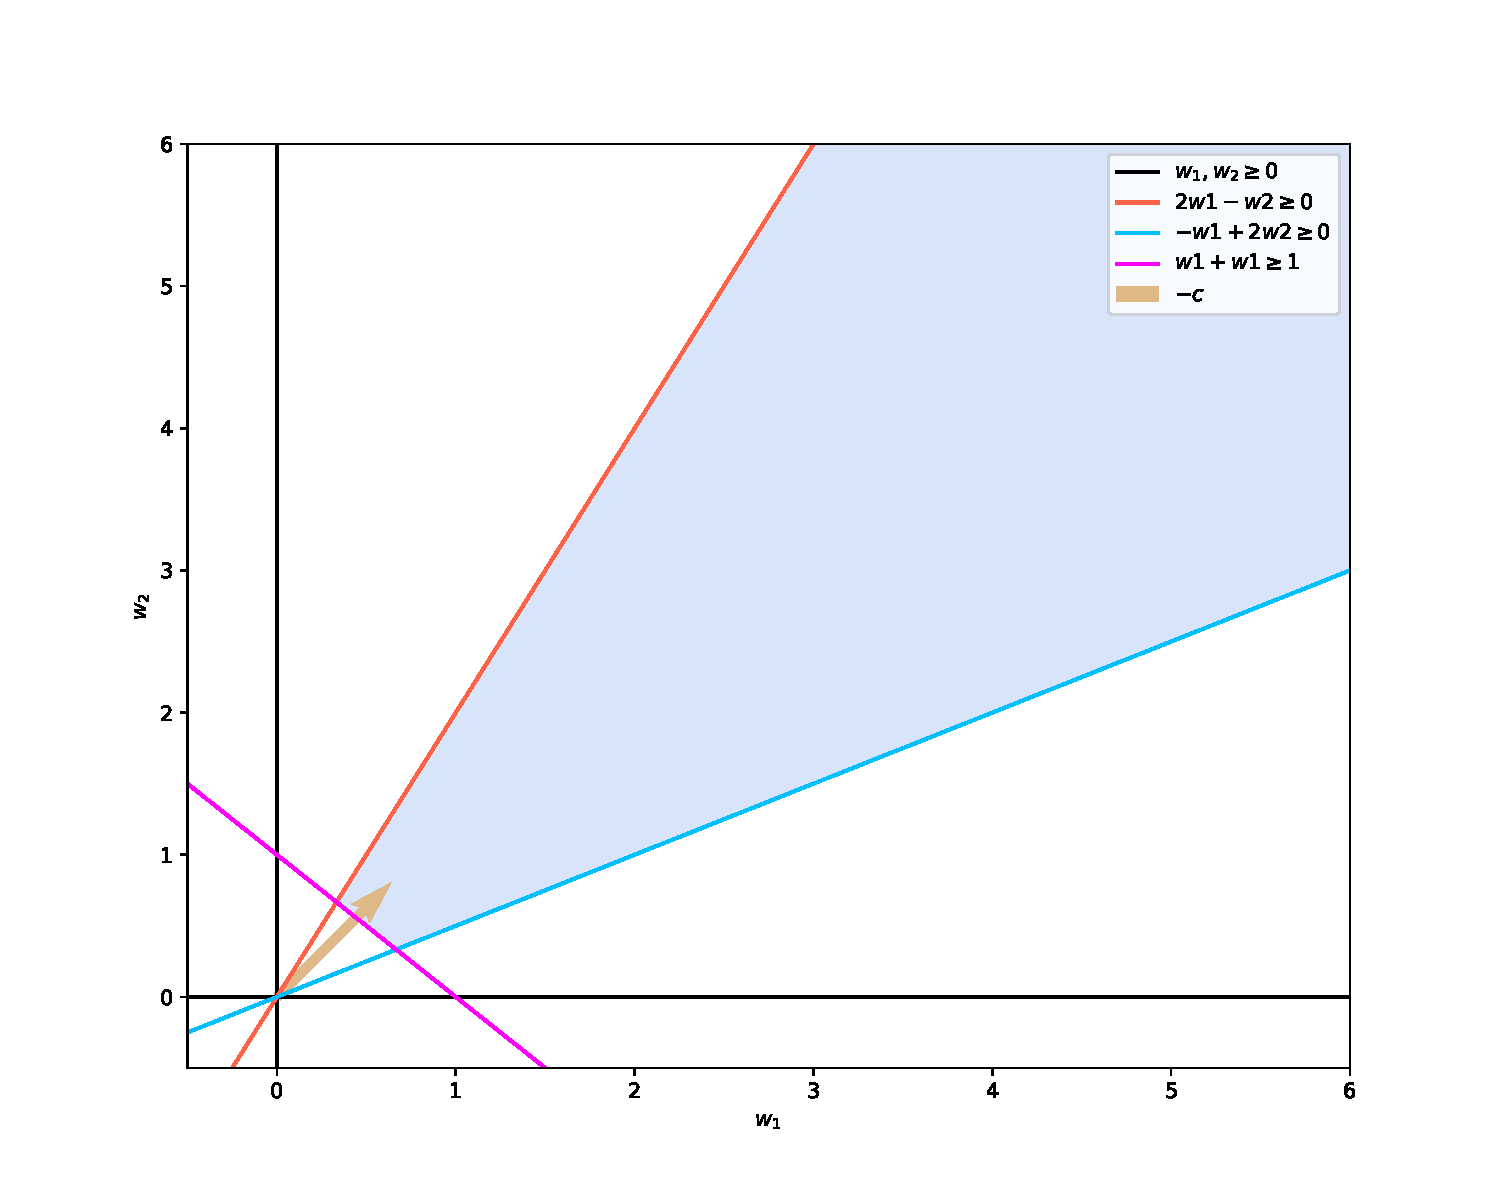
\includegraphics[scale=0.4]{Ej4}
  \caption{Región factible para el problema dual \(D\)}
  \label{fig:dual}
\end{figure}

Viendo estas restricciones y el vector \(-c\), podemos considerar para cada \(n \in \mathbb N\) la solución factible \(w_{n} = (n,n)^{T}\). Por tanto, los valores objetivo \(z_{n}^{*} = b^{T}w_{n} = -2n\), sucesión que tiende a menos infinito cuando \(n \to \infty\). Por esto, la solución del problema dual óptima es \textbf{no acotada}.\\

Haciendo ahora uso del Teorema \ref{th:dual}, como solo puede darse una de las opciones y aquí tenemos que uno de los problemas (el dual \(D\)) tiene una solución no acotada, el teorema nos dice que el problema primal \(P\) no tiene solución factible, como queríamos ver.


\end{document}
